\documentclass[12pt,a4paper]{article}

% Options possibles : 10pt, 11pt, 12pt (taille de la fonte)
%                     oneside, twoside (recto simple, recto-verso)
%                     draft, final (stade de développement)

\usepackage[utf8]{inputenc}   % LaTeX, comprends les accents !
\usepackage[T1]{fontenc}      % Police contenant les caractères français
\usepackage[french,english]{babel}  % Placez ici une liste de langues, la
                              % dernière étant la langue principale
\usepackage{textcomp}		  % pour le caractère ° and ~     
\usepackage[normalem]{ulem}   % pour rayer le texte
\usepackage{textgreek}		  % lettres grecs sans avoir à enter en math mode

%vector font
%\usepackage{cm-super}
 
%nested enumerate
\usepackage{enumitem}

%Abstract > Summary
\addto{\captionsenglish}{\renewcommand{\abstractname}{English and French abstract}}

%Figures                    
\usepackage{graphicx}
\graphicspath{ {Figures/} }
\usepackage{float} %To prevent floating figure
\usepackage[a4paper,left=2.5cm,right=2.5cm,top=3.0cm,bottom=3.0cm]{geometry}% Réduire les marges
\usepackage{titlesec} % Modifier le style des sections et chapitres

%Caption
\newcommand{\jcaption}[2]{\itshape \caption[#1]{\itshape #1#2}}

%Tableau
\usepackage{array,multirow,tabularx} % For table
\usepackage{slashbox} % Pour couper les tableaux avec une ligne diagonale
\usepackage[font=small,labelfont=bf]{caption}
\newcolumntype{L}[1]{>{\raggedright\let\newline\\\arraybackslash\hspace{0pt}}m{#1}}
\newcolumntype{C}[1]{>{\centering\let\newline\\\arraybackslash\hspace{0pt}}m{#1}}
\newcolumntype{R}[1]{>{\raggedleft\let\newline\\\arraybackslash\hspace{0pt}}m{#1}}

%paragraph
\setlength{\parindent}{4em}
\usepackage{indentfirst}
\setlength{\headheight}{15pt}
 
%list
\newenvironment{myitemize}
{ \begin{itemize}
	\setlength{\itemsep}{0pt}
	\setlength{\parskip}{0pt}
	\setlength{\parsep}{0pt} }
{ \end{itemize} }


\newenvironment{myenumerate}
{ \begin{enumerate}
	\setlength{\itemsep}{0pt}
	\setlength{\parskip}{0pt}
	\setlength{\parsep}{0pt} }
{ \end{enumerate} }
 
%Référence
\usepackage{hyperref }
%Référence perso
\newcommand{\refperso}[2]{\hyperref[#2]{#1~\ref*{#2}}}
%tilde
\newcommand{\tildep}[0]{\raise.17ex\hbox{$\scriptstyle\sim$}}

\usepackage{fancyhdr} % for use of \pageref{LastPage}
\pagestyle{fancy}

% Modifie le style par défaut
\fancypagestyle{IHA-fancy-style}{%
  \fancyhf{}% Clear header and footer
%  \fancyhead[L]{\leftmark}
%  \fancyhead[R]{\rightmark}
  \fancyhead[C]{\rightmark}
  \fancyfoot[L]{Jonhathan Pinon}
  \fancyfoot[R]{Page : \thepage}% Custom footer
  \renewcommand{\headrulewidth}{0.4pt}% Line at the header visible
  \renewcommand{\footrulewidth}{0.4pt}% Line at the footer visible
}

%Formules mathématiques centrées avec espace
\newenvironment{sp_equation}
{ \begin{equation}
 }
{ \end{equation} \smallskip }

%Appendix
\usepackage[titletoc,toc,page]{appendix}
%\renewcommand{\setthesubsection}{\Alph{section}}

%Scientific form in text mode
\newcommand{\sfnb}[2]{#1 $ \times$ 10 \textsuperscript{#2}}

%Math
\usepackage{amsmath,amssymb,mathrsfs}

\sloppy                       % Ne pas faire déborder les lignes dans la marge

\begin{document}
%

\begin{titlepage}

\vspace{5 cm}

\begin{center}

\Huge Final report for the peer-graded assignment of capstone project

\vspace{3 cm}

\Huge \textbf{Identifying the best places to open a French restaurant in Nagoya}

\vspace{2 cm}

\Large \textbf{by Jonhathan Pinon} \\

\vspace{2 cm}


\large 10/09/2019


\end{center}

\end{titlepage}

\clearpage
\tableofcontents
\phantomsection

\listoffigures


\pagestyle{IHA-fancy-style}


\section{Introduction}

\subsection{Background}


Nagoya is one of the largest cities in Japan. It has a population of over 2 millions and is situated in the middle-eastern part of Japan. In Japan, French cuisine is relatively popular. According to Foursquare data, there are about a hundred of French restaurants in Nagoya. Supposing that a chain of restaurants specialized in French cooking want to open new French restaurants in Nagoya, where would be the best places? 

\subsection{Problem}

The best place is the place that would attract the most customers. In this report, we define popularity as the number of customers. Ideally, we would need to identify, and ideally quantify, which factors are beneficial for attracting customers, and which are not. For example, we can expect the proximity of subway stations to substantially increase the popularity. On the other hand, we can expect that similar restaurants would decrease the popularity. However, the lack of data make quantifying the factors impossible. We will still attempt to estimate the best places using other means.

\subsection{Interest}

Such a map would obviously be very interesting for any group who wishes to open a restaurant. A restaurant popularity depends on its quality, but the location is still a major factor. To maximize potential income, choosing the place that would potentially attract the most customers is very important.

\section{Data description}

\subsection{Data sources}

Foursquare location data is the only data source. Foursquare provides the position of most restaurants, train stations, subway stations, and other venues in Nagoya. The location of all venues in Nagoya listed by Foursquare, along with their category, will be our main data during this study. We could further increase the amount of data using other API such as Google Maps's API, but we judged it would create more inconsistently than benefits due to the different nature of the data (for example, the categories are not the same). Henceforth, we limited our source to Foursquare.

\medskip

In addition, Foursquare provides stats about each venue such as the number of visitors currently at the specified venue. By collecting the number of users at a specific venue over the course of several weeks, we could get an estimate of its popularity. Unfortunately, in the scope of this course, we did not have enough time to collect enough data.  Foursquare allowed developers to get the total number of visits of any venue by getting the details of that venue, thanks to the response field \textit{checkinsCount}, but since April 2018, this no longer possible (reference 1).

\subsection{Dataframes}

Almost all data are stocked in dataframes, objects of the python library pandas. Some data were stocked temporary in lists and series for the sake of coding.
All relevant data from Foursquare were stocked into dataframes. The dataframe that were used to stock the data are:

\begin{itemize}
  \item french\_venues that contains all French restaurants in Nagoya (Figure \ref{french_df}).
  \item nagoya\_venues\_food that contains all restaurants in Nagoya (except French restaurants).
  \item nagoya\_venues\_transport that contains all transport venues in Nagoya.
  \item nagoya\_venues\_longstay that contains all workplace and residence related venues in Nagoya.
  \item nagoya\_venues\_shortstay that contains all shops, recreation, hobbies, park, art related venues in Nagoya (Figure \ref{nagoya_shortstay_df}).
\end{itemize}

\begin{figure}[ht]
	\begin{center}
			  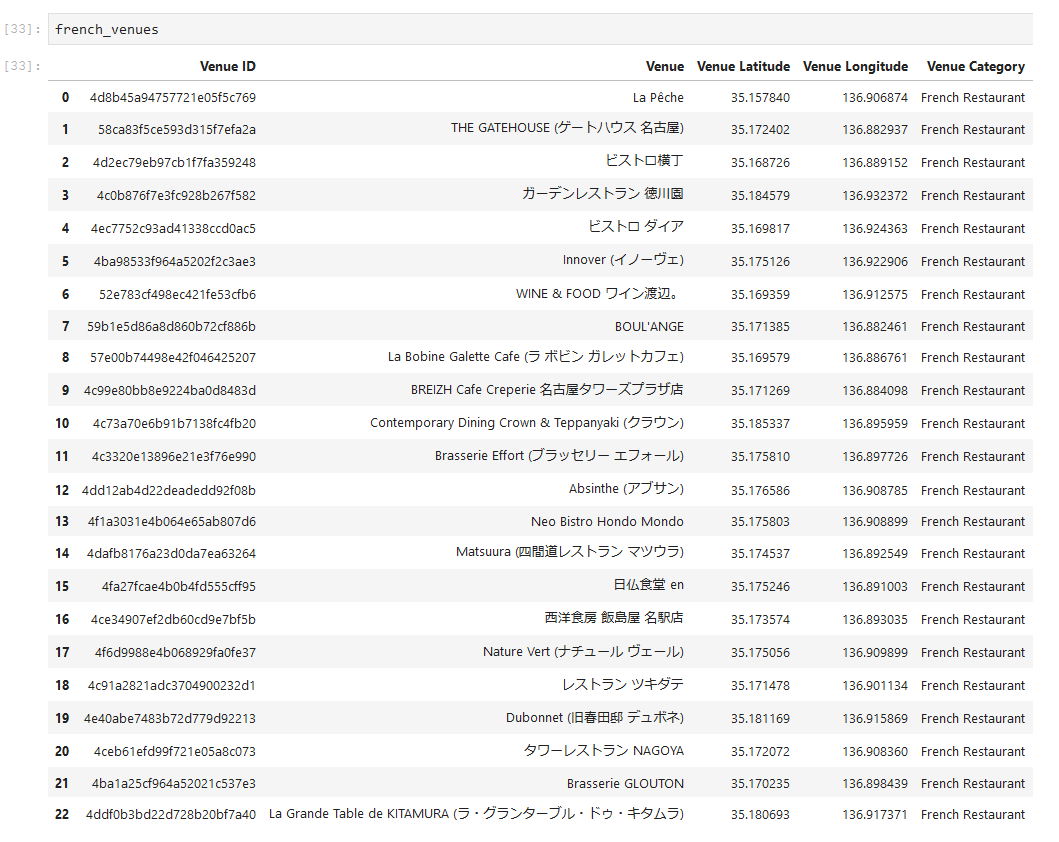
\includegraphics[width=15cm]{french_venues_df.png}
	\end{center}
	\caption [\itshape First part of the dataframe listing all French restaurants in Nagoya]{\itshape First part of the dataframe listing all French restaurants in Nagoya}	
	\label{french_df}
\end{figure}

\begin{figure}[ht]
	\begin{center}
			  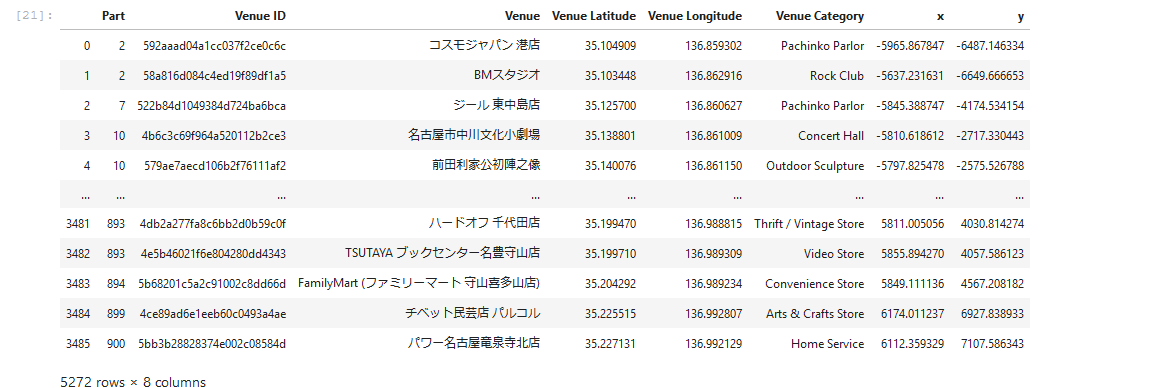
\includegraphics[width=15cm]{shortstay_venues_df.png}
	\end{center}
	\caption [\itshape First part of the dataframe listing all 'short stay' venues in Nagoya]{\itshape First part of the dataframe listing all 'short stay' venues in Nagoya}	
	\label{nagoya_shortstay_df}
\end{figure}


\subsection{Data cleaning}

In the case of the dataframe containing the French restaurants, \textit{french\_venues}, directly after the construction of the dataframe from Foursquare data, some venues are not classified as French restaurants. This is because in Foursquare, venues can have several categories. When searching for all venues belonging to a certain category, Foursquare will pick all venues that contains that specific category among all their categories. Then, in our script, for each venue, we select its first category as its category which will be later stocked in the dataframe. As that first category may not necessarily be 'French restaurant', we manually reassign the category 'French restaurant' to all venues in \textit{french\_venues}.

\medskip

In the case of the dataframes containing the other kind of venues around French restaurants in Nagoya, due to how we collected the data, there are thousands of duplicates. We remove them by dropping the duplicate rows from the dataframe. The construction of that dataframe, \textit{nagoya\_venues}, is explained in details in the following section. We remove all French restaurants in those dataframes. 

\section{Methodology}

\subsection*{Principe}

Our final goal is to get a list of the best places to open a French restaurant in Nagoya. As mentioned above, we cannot measure the popularity of a restaurant using Foursquare data. Consequently, it is nearly impossible to find out and measure what factors, related to its geographical position, make a restaurant popular. 

\medskip

Let us think from another perspective. Let us assume the owners of the already existing French restaurants thought thoroughly where they should open a French restaurant. Let us assume that the previous French restaurants were opened at \textit{good places}. Then by analyzing the geographical details of each French restaurant, we can estimate what kind of places French restaurants tend to be opened. In other words, what are the best places to open a French restaurant. By \textit{geographical details}, we mean the venues surrounding the French restaurants. For example, if we discover that French restaurants tend to be close to subway stations and far away from other restaurants, then we find the best places in Nagoya by looking at which points the distances from subway stations are minimized while the distances from other restaurants are maximized. 

\medskip

This is the general idea of our methodology. Due to the limited computing power, we cannot look at each possible point (i.e: set of longitude and latitude) in Nagoya. We decided to limit our study to a grid of 30*30 points in an area which contains all French restaurants in Nagoya. There are thus 900 points in the grid. The grid is shown on Figure \ref{nagoya_grid}. The red circle is the area studied, which was defined so as to contain all French restaurants in Nagoya and their surrounding venues. The meaning of the blue circles is explained in the next subsection. 

\begin{figure}[ht]
	\begin{center}
			  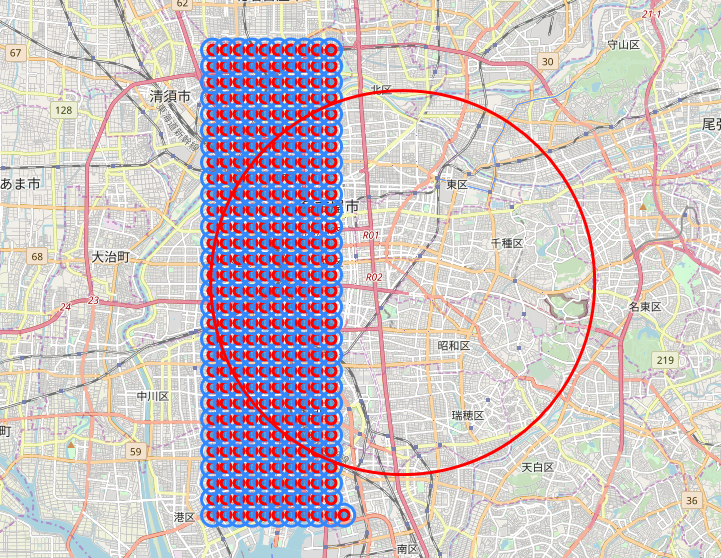
\includegraphics[width=15cm]{nagoya_grid.png}
	\end{center}
	\caption [\itshape Division of Nagoya into a 30*30 grid]{\itshape Division of Nagoya into a 30*30 grid}	
	\label{nagoya_grid}
\end{figure}

\medskip

For each point in the grid, we will calculate a \textit{similarity distance}. The lower it is, the more this area is similar to the other areas with French restaurants. In other words. the more recommended it is to open a restaurant at that place. This \textit{similarity distance} is the the weighted sum of several 'distances'. They measure the similarity of the area with the other areas with French restaurants, with regards to the numbers of restaurants, short stay venues, long stay venues and transport venues.

\begin{multline}
	\textbf{similarity distance}_{i} =  \Sigma_{j} \quad a_1 (pfood_{fr,j} - pfood_{a,i})^2  \\ + a_2 (ptrans_{fr,j} - ptrans_{a,i})^2 
	+ a_3  (plgstay_{fr,j} - plgstay_{a,i})^2  \\ + a_4 (pshstay_{fr,j} - pshstay_{a,i})^2 + a_5 (nvenues_{fr,j} - nvenues_{a,i})^2
\end{multline}

\medskip

\begin{itemize}
  \item $\textbf{similarity distance}_{i}$ is the similarity distance of the area i, belonging to the 30*30 grid (lower = more similar).
  
  \item $a_1$ is a coefficient that weights the distance relative to restaurant venues. It will be adjusted later.
  \item $pfood_{fr,j}$ is the proportion of restaurant venues compared to all other kind of venues, in a 150 meters around the French restaurant j.
  \item $pfood_{a,i}$ is the proportion of restaurant venues compared to all other kind of venues, in a 150 meters around the area i.
  
  \item $a_2$ is a coefficient that weights the distance relative to transport venues. It will be adjusted later.
  \item $ptrans_{fr,j}$ is the proportion of transport venues compared to all other kind of venues, in a 150 meters around the French restaurant j.
  \item $ptrans_{a,i}$ is the proportion of transport venues compared to all other kind of venues, in a 150 meters around the area i.
  
  \item $a_3$ is a coefficient that weights the distance relative to long stay venues. It will be adjusted later.
  \item $plgstay_{fr,j}$ is the proportion of long stay  venues compared to all other kind of venues, in a 150 meters around the French restaurant j.
  \item $plgstay_{a,i}$ is the proportion of long stay  venues compared to all other kind of venues, in a 150 meters around the area i.
  
  \item $a_4$ is a coefficient that weights the distance relative to short stay venues. It will be adjusted later.
  \item $shstay_{fr,j}$ is the proportion of short stay venues compared to all other kind of venues, in a 150 meters around the French restaurant j.
  \item $shstay_{a,i}$ is the proportion of short stay venues compared to all other kind of venues, in a 150 meters around the area i.
  
  \item $a_5$ is a coefficient that weights the distance relative to the number of all venues. It will be adjusted later.
  \item $nvenues_{fr,j}$ is the number of all venues in a 150 meters around the French restaurant j.
  \item $nvenues_{a,i}$ is the number of all venues in a 150 meters around the area i.

\end{itemize}

We choose 150 meters as the limit because we suppose that beyond 150 meters, the impact of other venues become negligible compared to the impact of the closer venues .

\medskip

Intuitively, the impact of the nearby transports seems larger than the impact of short stay and long stay venues. The number of shops (short stay) should impact the popularity of French restaurant differently than the number of offices (long stay) nearby too. This is why we separated the 3 above types of venues, with 3 coefficients $a_2$, $a_3$ and $a_4$.

\medskip

The presence of nearby restaurants may not be beneficial because of competition. Hence, we used a different coefficient, $a_1$, for food-related venues.

\medskip

The proportion of a certain kind of venues versus the number of all venues may matter more than the absolute number of that kind of venues. For example, an area with 10 restaurants and 20 transport venues seems more attractive than an area with 20 restaurants and 10 transport venues. This is why we are comparing proportions rather than absolute numbers. This way, we are less biased against areas with a small amount of venues. To keep all information, we still compare the absolute number of venues, weighted by $a_5$.

\medskip

We will use an optimization algorithm to find the best coefficients.

\medskip

After we calculate the similarly distance for every area in the grid, we will rank the areas according to the distance. The areas with the lowest distance are the most recommended areas.

\subsection{Preparation of the data}

The collection of all French restaurants in Nagoya is straightforward. We run a single request to Foursquare API to get the list of all venues that are classified as \textit{French restaurant}. The latitude and the longitude of the center of the circle where the venues are explored are obtained through the python libray \textit{geopy}.

\medskip

The collection of all venues, which are NOT French restaurants, is more complex. One of the limits of Foursquare API is that a single request, to explore the venues around a place, only gives back at most 100 venues. However, there are certainly more than 100 venues in Nagoya. To get as many venues as possible, we split Nagoya, or more precisely the area around the French restaurants, into 900 parts, in a 30*30 grid. The grid is the same grid referenced in Figure \ref{nagoya_grid}. Then for each area, we make a call and get the list of all venues in that area. The blue circles in the Figure represent the size of each area. Let us notice that the surface inside the red circle, which contains all French restaurants in Nagoya, is covered by the blue circles. Thanks to this division of Nagoya, we can get most of the venues around French restaurants by making 900 calls to Foursquare API.

\medskip

Of course, collecting the venues this way will generate a lot of duplicates. Indeed, each point inside the red circle is covered by several blue circles. To clean our data, we drop the duplicates in \textit{nagoya\_venues}.

\medskip

The calculation of the \textit{similarity distance} will involve hundreds of thousands of mathematical operations. The distance between each French restaurant and each venue in Nagoya will be calculated. We can calculate the distance between two points on Earth using the Haversine formula, but this formula involves trigonometric functions which would make the computational time far too long. To accelerate as much as possible the calculation of the \textit{similarity index}, we will first calculate the position of all venues (including French restaurants) in a local Cartesian system. The center of this coordinate system will the center of the red circle, shown on Figure \ref{nagoya_grid}. To transform the latitude and longitude into Cartesian coordinates, we use the formula described in reference 2. This formula is derived from the Equirectangular approximation. The formula is as follow:

\begin{equation}
	x = R * (lgt - lgt_0) * cos (lat_0)	
\end{equation}

\begin{equation}
	y = R * (lat - lat_0)
\end{equation}

where:

\begin{itemize}
  \item $R$ is the radius of Earth (~6373 km)
  \item $lgt$ is the longitude in radians of the given point
  \item $lat$ is the latitude in radians of the given point
  \item $lgt_0$ is the longitude in radians of the origin
  \item $lat_0$ is the latitude in radians of the origin
\end{itemize}
 
The Equirectangular approximation is a good enough approximation considering the distances involved. We verified this hypothesis by comparing the distances calculated using this approximation to the distances calculated using the Haversine formula.

\medskip

All venues in \textit{french\_venues} and the other dataframes have now their coordinates in the local Cartesian system.
 
\subsection{Calculation of the similarity distance and the F1 score}

Let us describe step by step how we calculate the similarity distance and then the f1 score:

\begin{enumerate}

	\item Make the dataframe containing all french restaurants in Nagoya

	\item Make the dataframe containing all restaurants / transport venues / long stay venues / short venues in Nagoya. Take out all French restaurants.
	
	\item Clean the dataframes : delete duplicates. Change the category of each venue to the first category listed (because one venue can have several categories).
	
	\item Calculate the x and y local Cartesian coordinates to greatly accelerate the calculations later.
	
	\item For each french restaurant in the French dataframe, calculate the total number of venues, the proportion of other restaurants, transport venues, short stay venues and long stay venues in a 150 meter radius.
	
	\item For each area in the grid, calculate the total number of venues, and the aforementioned proportions in a 150 meter radius. Those data are stocked in the dataframe nagoya\_grid\_df. Delete rows that have NaN values (which happens if there is no restaurant / transport / other venues in the 150 meter radius).
	
	\item Calculate for each area the similarity distance using the formula above.
	
	\item For each area in the grid, check if there is a French restaurant. Get the number, \textit{nb\_areas\_with\_fr} of different areas with at least one French restaurant. This number is smaller than the total number of French restaurants because there can be more than one French restaurants per area.
	
	\item Sort each area by their similarity distance. The \textit{nb\_areas\_with\_fr} first areas with the smallest distance will be marked as having a 'predicted' French restaurant.

	\item Check if the areas that have predicted French restaurants also have real French restaurants (true positive). Do the same for true negative, false positive and false negative. Calculate the F1 score (calculated automatically using the function f1\_score from the sklearn library).
	
	\item  The calculation of the similarity distance was done with one set of $a_k (1<k<=5)$. To try to get the best results, reiterate the steps from the similarly distance calculation with different $a_k$. The $a_k$ will be chosen automatically by the optimization algorithm. Here, we decided to use the least square method and the Broyden–Fletcher–Goldfarb–Shanno (BFGS) algorithm. The goal is to get the highest F1 score.

\end{enumerate}

\section{Results}

\subsection{Preliminary results}

Before applying the model, we explored the data with pandas. We plotted the histograms of the distributions of:

\begin{itemize}

	\item Other restaurants in a 150 meter radius around French restaurant : Figure \ref{hist_food}.
	\item Transport venues in a 150 meter radius around French restaurant : Figure \ref{hist_transport}.
	\item Long stay venues in a 150 meter radius around French restaurant : Figure \ref{hist_longstay}.
	\item Short stay venues in a 150 meter radius around French restaurant : Figure \ref{hist_shortstay}.

\end{itemize}

For the four distributions, we see French restaurants tend to be in areas with few other venues. 
In fact, the more venues there are, the less likely there are French restaurants ... Or at least, this is what we could believe if we just look at the plots. The truth is more complicated because the number of low venue populated areas outnumber greatly the number of high venue populated areas. Hence, it is expected that we find more French restaurants in low venues populated areas, just because there are much more low populated areas.

\medskip

The distribution of restaurants is clearly different from the other distributions. It is not as left-sided. It shows that the presence of French restaurants is more strongly correlated with the presence of other restaurants. Competition does not seem to matter. We can explain this by the fact that an area with a lot of restaurants is very attractive for a French restaurant, like any restaurant. Otherwise, there would not be a lot of restaurants in that area in the first place. 

\medskip

Considering the distributions of transport, long stay and short stay related venues are similar, it may be more efficient to group them together in the similarly distance equation (i.e: same coefficient). But for the sake of completeness, we decided to keep them separated. 

\begin{figure}[ht]
	\begin{center}
			  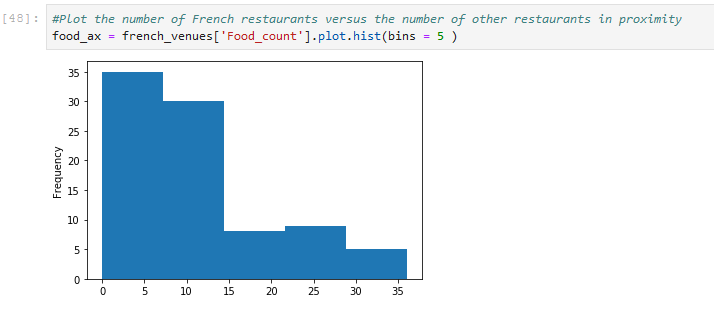
\includegraphics[width=10cm]{hist_food.png}
	\end{center}
	\caption [\itshape Distribution of the number of restaurants around French restaurants]{\itshape Distribution of the number of restaurants around French restaurants}	
	\label{hist_food}
\end{figure}

\begin{figure}[ht]
	\begin{center}
			  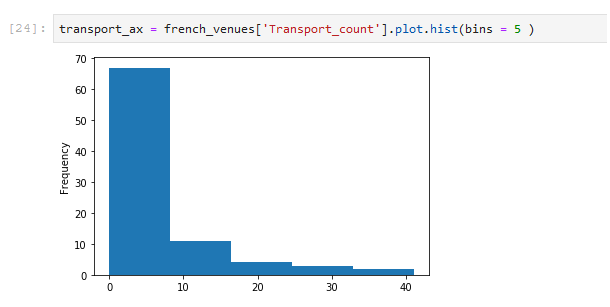
\includegraphics[width=10cm]{hist_transport.png}
	\end{center}
	\caption [\itshape Distribution of the number of transport venues around French restaurants]{\itshape Distribution of the number of transport venues around French restaurants}	
	\label{hist_transport}
\end{figure}

\begin{figure}[ht]
	\begin{center}
			  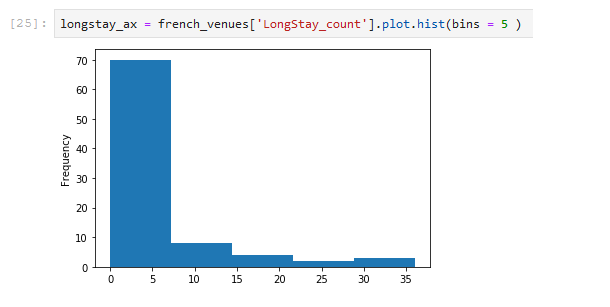
\includegraphics[width=10cm]{hist_longstay.png}
	\end{center}
	\caption [\itshape Distribution of the number of long stay venues around French restaurants]{\itshape Distribution of the number of long stay venues around French restaurants}	
	\label{hist_longstay}
\end{figure}

\begin{figure}[ht]
	\begin{center}
			  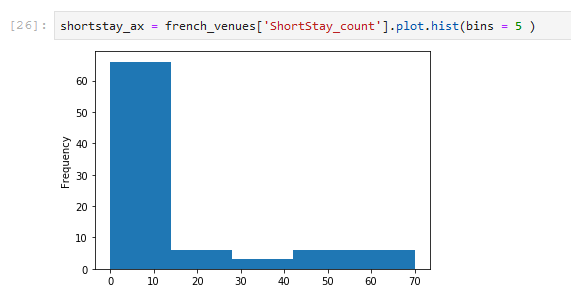
\includegraphics[width=10cm]{hist_shortstay.png}
	\end{center}
	\caption [\itshape Distribution of the number of short stay venues around French restaurants]{\itshape Distribution of the number of short stay venues around French restaurants}	
	\label{hist_shortstay}
\end{figure}

\subsection{Model results}

To test the accuracy of our model, we divided the dataframe containing the French restaurants into two parts.
One part for training the model (finding the coefficients $a_k$ giving the highest f1 score) and one part to test the model.

\medskip

We used the least square algorithm and the Broyden–Fletcher–Goldfarb–Shanno (BFGS) algorithm from the scipy library to optimizes the model.

\medskip

The initial vector was:

\begin{itemize}
	\item $a_1 = 1$
	\item $a_2 = 1$
	\item $a_3 = 1$
	\item $a_4 = 1$
	\item $a_5 = 0.01$
\end{itemize}

We supposed the impact of food-related venues was the same as the impacts of the other kinds of venues.
We assigned a coefficient 100 times lower for the impact of the absolute number of venues, because in the case of the proportions, the distance ($(plgstay_{fr,j} - plgstay_{a,i})^2$) should be between 0 and 1. Whereas, in the case of the absolute number of nearby venues, the distance ($nvenues_{fr,j} - nvenues_{a,i})^2$ should be between 0 and ~10,000 (in average, between 100 and 1000).

\medskip

Despite trying both algorithm, we failed to find a better vector than the one above. The two algorithms stopped (successfully) at the first iteration. We tried several different initial vectors, such as [1,1,1,1,0.0001], but no matter what, the algorithms stopped at the first iteration. The f1 score was slightly worse when we tried other initial vectors (~0.375 instead of ~0.406 for example). The function that gives the f1 score, which we tried to optimize, is non-linear and extremely complex. There are about 80*5 (French restaurants) + 900*5 (grid of Nagoya) independent variables. This is why the algorithm failed to find a better vector.

\medskip

The f1 score on the training set was 0.40625.

\medskip

The f1 score on the test set was  0.1212.

\medskip

The f1 score on the complete (training + test) set was  0.3875. 
The worst score is due to the fact there can be more than one French restaurant per area.

\medskip

The maps showing the true positives (in green), true negatives (in blue), false positives (in red) and false negatives (in yellow) in the three cases are shown in Figure \ref{map_training} (training set), Figure \ref{map_test} (test set) and Figure \ref{map_complete} (complete set).

\begin{figure}[ht]
	\begin{center}
			  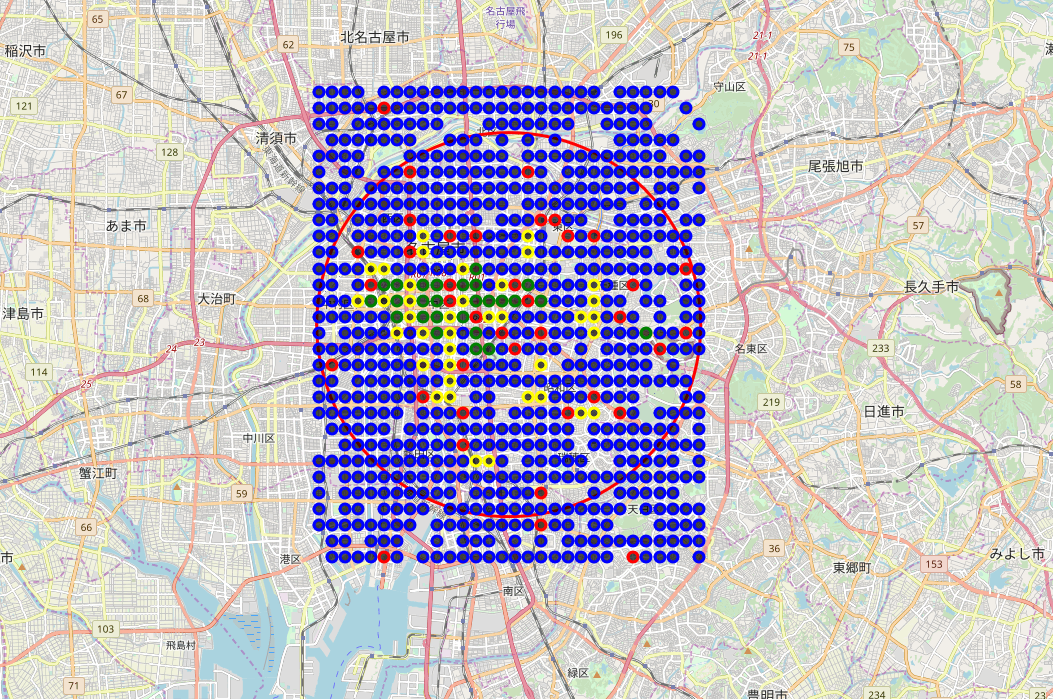
\includegraphics[width=15cm]{model_result_map_training.png}
	\end{center}
	\caption [\itshape Grid of Nagoya showing true positives, true negatives, false positives and false negatives on the training set]{\itshape Grid of Nagoya showing true positives, true negatives, false positives and false negatives on the training set}	
	\label{map_training}
\end{figure}

\begin{figure}[ht]
	\begin{center}
			  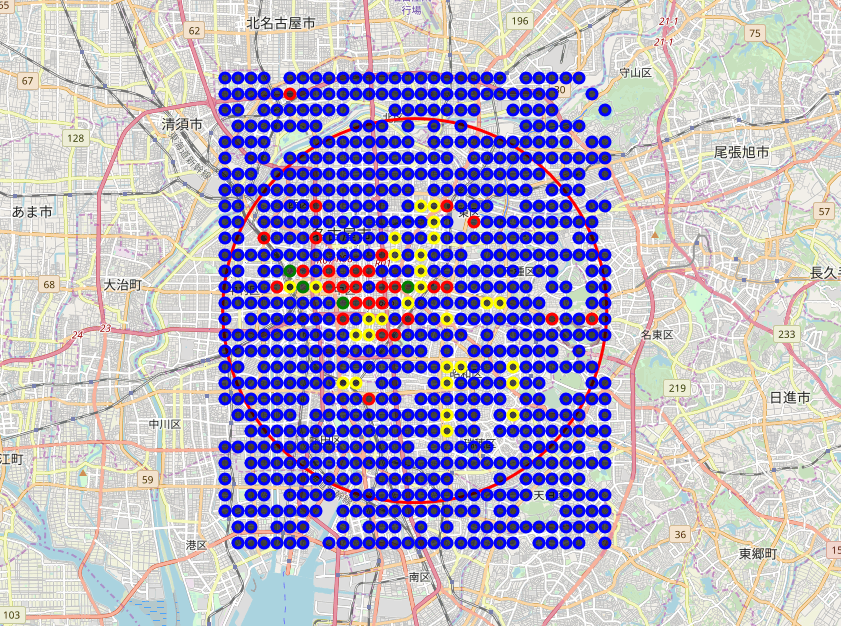
\includegraphics[width=15cm]{model_result_map_test.png}
	\end{center}
	\caption [\itshape Grid of Nagoya showing true positives, true negatives, false positives and false negatives on the test set]{\itshape Grid of Nagoya showing true positives, true negatives, false positives and false negatives on the test set}	
	\label{map_test}
\end{figure}

\begin{figure}[ht]
	\begin{center}
			  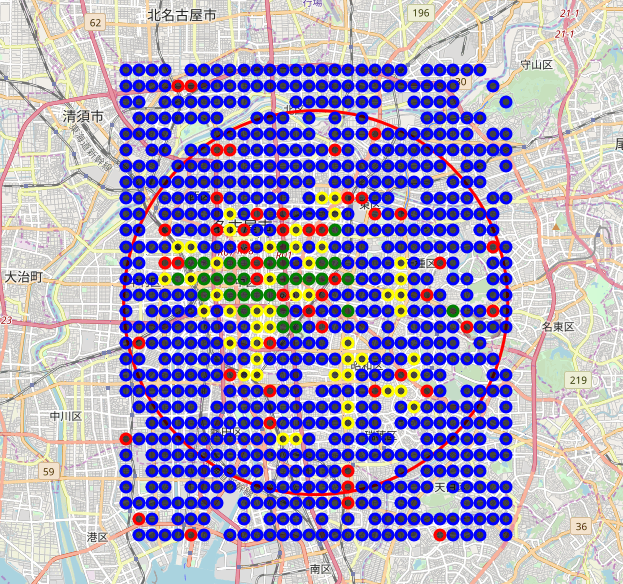
\includegraphics[width=15cm]{model_result_map_complete.png}
	\end{center}
	\caption [\itshape Grid of Nagoya showing true positives, true negatives, false positives and false negatives on the complete set]{\itshape Grid of Nagoya showing true positives, true negatives, false positives and false negatives on the complete set}	
	\label{map_complete}
\end{figure}

\section{Discussion}

\subsection{Accuracy of the model}

The f1 score is bad (~0.40). It would be even worse if there was not a certain bias in the model. We calculated the similarity distance for each area. Then we took the \textit{nb\_areas\_with\_fr} areas with the smallest distance. \textit{nb\_areas\_with\_fr} is the number of areas with at least one (true) French restaurant. This means that no matter what, the model is guaranteed to predict as many areas with French restaurants as there are in reality:

\begin{equation}
	\textit{true positive + false positive} =  \textit{real number of areas with French restaurant}
\end{equation}

\begin{equation}
	\textit{true negative + false negative} =  \textit{real number of areas without French restaurant}
\end{equation}

Despite the low score, the model is better than random predictions. We calculated the average f1 score if the list of predicted areas with French restaurants was generated totally randomly, instead of being the list of the areas with the smallest similarity distance. We ran 2000 simulations and averaged the f1 score.

\medskip

The f1 score obtained was about 0.10. Although the f1 score of our model is bad, it is still 4 times higher than the random f1 score. The model is considerably better than random guesses. 

\medskip

Let us go back to the original question : where would be the best places to open a French restaurant? We need to look at the false positives (red, Figure \ref{map_complete}) to answer this question. The false positives at the edge of the map seem to be outlier and thus should be ignored. The areas with several consecutive red points look promising, especially if there are no true or false negatives nearby. Although the model is bad, it is not random. It proposes areas that are similar to areas with French restaurants. If it proposes several areas without yet existing restaurants, it means there are potentially a market with few competition in those areas.

\subsection{Limit of the study}

The absence of data on the popularity of the venues was a major problem. If we could get the number of visits of every venues in Nagoya, then we would be able to check what factors impact the popularity of French restaurants. Does the number of nearby restaurants increase in average the number of visits? Does the presence of nearby French restaurants decrease in average the number of visits? Such questions could have been answered if we had access to those data.

\medskip

Foursquare does not list ALL venues in Nagoya. In fact, based on my experience in Nagoya, I would stay about 20\% at most are shown. Besides, Foursquare's API is inconsistent . Concretely, let us say we find all French restaurants inside a 1 kilometer circle. Let us say we get 80 results. Then, if we search all French and Italian restaurants inside that same area, by calling API one time, we may find just 60 French restaurants instead of 80!

\section{Conclusion}

The goal of the study is to find the best places to open a French restaurant in Nagoya. This question is very important for any chain or individual who wishes to open a French restaurant in Nagoya. To answer this problem, we used exclusively Foursquare API. Unfortunately, the lack of data regarding the number of visits for each venue forced us to devise indirect, and thus very complex, ways to predict the best areas. The underlining principle is that previous shops owners opened their restaurants in the best places. Hence, looking for areas similar to the current areas with French restaurants should show us good areas to open a new restaurant.

\medskip

To find those areas, we first defined a 'similarity distance'. This distance represents how similar an area is compared to the average area with French restaurants with regards to the proportion of restaurants, transports, long stay venues, short stay venues and total number of nearby venues. The result showed the model was inaccurate. The f1 score on the complete set was just 0.4. Furthermore, the machine algorithms we tried failed to find a better initial vector due to the complexity of the model. Even so, we demonstrated it was better than random guesses, and thus could be used to estimate where to open a French restaurant. 

\medskip

Much more useful models could be built if we had access to the number of visits. Even with the data we collected, we believe better models could be built. For example, we chose to count all restaurants, shops and so on around French restaurants in a 150 meter radius. This limit, 150, should have considerable impact on the result. We also could find a better vector. More importantly, we could build a new model based on a new equation, hopefully simpler and more intuitive. 

\medskip

The results are unsatisfactory from a business point of view. But considering the scope of this project (one person, 30 hours, application of data science), I personally believe this study demonstrates the skills learned from the courses of IBM Data Science Professional Certificate.

\section*{References}

\begin{enumerate}
  \item https://developer.foursquare.com/docs/announcements\#start-up-tier-launch
  \item http://www.movable-type.co.uk/scripts/latlong.html
\end{enumerate}


\end{document}


